\subsection{A 贡献者名单}\label{a-contributions}

贡献者名单按姓氏字母顺序排列。

{\def\LTcaptype{none} % do not increment counter
\begin{longtable}[]{@{}|l|l|l|l|@{}}
\toprule\noalign{}
\endhead
\bottomrule\noalign{}
\endlastfoot
\hline
Tongtong Bai & Fuxuan Gao & Aidi Li & Shaoguang Mao \\
\hline
Yifan Bai & Hongcheng Gao & Cheng Li & Yuan Mei \\
\hline
Yiping Bao & Jingyue Gao & Chengyuan Li & Xin Men \\
\hline
M. C. & Tong Gao & Cong Li & Minqing Ni \\
\hline
Jianfeng Cai & Weijia Gao & Fang Li & Yixuan Niu \\
\hline
Xinyuan Cai & Shangyi Geng & Guanyu Li & Siyuan Pan \\
\hline
Peizhou Cao & Jie Gong & Haoyang Li & Shujun Peng \\
\hline
Yuxuan Cao & Linhu Gong & Jia Li & Zhangyang Qi \\
\hline
Ziwei Chai & Shengao Gong & Junxiong Li & Ruoyu Qin \\
\hline
Y. Charles & Xiaochen Gong & Lei Li & ZeChao Qin \\
\hline
H.S. Che & Qizheng Gu & Letian Li & Zeyu Qin \\
\hline
Guanduo Chen & Yicheng Gu & Lincan Li & Haiquan Qiu \\
\hline
Guangyu Chen & Shuhao Guan & Weihong Li & Jianxin Qiu \\
\hline
Guanzheng Chen & Haiqing Guo & Wentao Li & Jiezhong Qiu \\
\hline
Huarong Chen & Shiqi Guo & Xintong Li & Bowen Qu \\
\hline
Jia Chen & Xiang Guo & Yang Li & Yuhao Qu \\
\hline
Jianlong Chen & Zhengyan Guo & Yishen Li & Zeyu Shang \\
\hline
Jun Chen & Beixi Hao & Yiwei Li & Youbo Shao \\
\hline
Kexin Chen & Wenxin Hao & Yuxiao Li & Han Shen \\
\hline
Peng Chen & Xiaoru Hao & Zhaowei Li & Jincheng Shi \\
\hline
Ruijue Chen & Dailan He & Zhaoxi Li & Juanfeng Shi \\
\hline
Wentao Chen & Haotian He & Zheming Li & Lidong Shi \\
\hline
Xin Chen & Lehan He & Zhengxiao Li & Shengyuan Shi \\
\hline
Yang Chen & Qi He & Zhiyuan Li & Wingchun Siu \\
\hline
Yanru Chen & Weiran He & Jiawei Lin & Pengwei Song \\
\hline
Yifei Chen & Xinran He & Xiaohan Lin & Xiaoxi Song \\
\hline
Yingjiang Chen & Xinyi He & Yibo Lin & Jianlin Su \\
\hline
Yuankun Chen & Yibo He & Zichao Lin & Yunfeng Su \\
\hline
Yujie Chen & Yunjia He & Ziyan Lin & Zhaochen Su \\
\hline
Yutian Chen & Chao Hong & Bill Liu & Lin Sui \\
\hline
Zhirong Chen & Tiange Hong & Boxiao Liu & Jingsong Sun \\
\hline
Dazhi Cheng & Hao Hu & Chuan Liu & Junyao Sun \\
\hline
Yean Cheng & Jiaxi Hu & Liang Liu & Shaoning Sun \\
\hline
Jialei Cui & Ruikun Hu & Shaowei Liu & Shuzhe Sun \\
\hline
Jingbing Cui & Weiming Hu & Shudong Liu & Tongyu Sun \\
\hline
Anqi Dai & Yangyang Hu & Shuran Liu & Yujun Sun \\
\hline
Jiaqi Deng & Zhenxing Hu & Tianwei Liu & Yunpeng Tai \\
\hline
Hao Ding & Liang Hua & Weizhou Liu & Chuning Tang \\
\hline
Rui Ding & Jinbin Huang & Yangyang Liu & Heyi Tang \\
\hline
Shaofeng Ding & Ke Huang & Yanming Liu & Sirui Tang \\
\hline
Mengfan Dong & Ruiyuan Huang & Yibo Liu & Zecheng Tang \\
\hline
Mengnan Dong & Siying Huang & Yipeng Liu & Chaoran Tian \\
\hline
Yuhao Dong & Weixiao Huang & Zhengying Liu & Rongpeng Tian \\
\hline
Yuxin Dong & Yan Huang & Zhiheng Liu & Yu Tian \\
\hline
Ang\textquotesingle ang Du & Zhengjie Huang & Enzhe Lu & Wei Tu \\
\hline
Chenzhuang Du & Zhiqi Huang & Haoyu Lu & Chensi Wang \\
\hline
Dikang Du & Chaobo Jia & Linqiang Lu & Chuang Wang \\
\hline
Jusen Du & Yutong Jiang & Tingzhan Lu & Chunjie Wang \\
\hline
Yulun Du & Zhejun Jiang & Zhiyuan Lu & Dinglu Wang \\
\hline
Yu Fan & Zuoyou Jiang & Aotian Luo & Feng Wang \\
\hline
Jing Feng & Wenyi Jin & G. Luo & Hailong Wang \\
\hline
Qiulin Feng & Xinyi Jin & Junyu Luo & Haiming Wang \\
\hline
Yichen Feng & Yu Jing & Yifan Luo & Hao Wang \\
\hline
Kelin Fu & Huanjun Kong & B. Lyu & Hao Wang \\
\hline
Qiang Fu & Guokun Lai & Wenzhou Lyu & Huaqing Wang \\
\hline
\end{longtable}
}

Hui Wang Jiayi Wang Jinglong Wang Jinhong Wang Jiuzheng Wang Linian Wang
Shaobo Wang Shenzhi Wang Shuyi Wang Si Wang Siyuan Wang Tianfu Wang
Wenjue Wang Xingran Wang Xinmei Wang Xinyuan Wang Xusheng Wang Yalin
Wang Yangkun Wang Yao Wang Yaoyu Wang Yejie Wang Yiqin Wang Yucheng Wang
Yuzhi Wang Zhaoji Wang Zhaowei Wang Zhengtao Wang Zhenhao Wang
Zhongsheng Wang Zifan Wang Chu Wei Ming Wei Shouxin Wei Zichen Wen Fan
Wu Haoning Wu Rucong Wu Wenhao Wu Xiaoxue Wu Yingcong Wu Yongqi Wu Yuxin
Wu Zijian Wu Xinglang Xian Chenxuan Xiang

Yuye Xiang Bocheng Xiao Chenjun Xiao Xin Xiao Jin Xie Xiaotong Xie
Yifeng Xie Zhe Xie Bowei Xing Yiming Xiong Baosheng Xu Boyu Xu Jiale Xu
Jianfan Xu Jing Xu Jinjing Xu L.H. Xu Qingtao Xu Shuyao Xu Suting Xu
Tiantian Xu Tianxiang Xu Weixin Xu Xinran Xu Yangchuan Xu Ye Xu Yueni Xu
Ziyao Xu Haonan Xue Junjie Yan Yaoyao Yan Fan Yang Guangyao Yang Hao
Yang Junwei Yang Ruoyu Yang Wenjie Yang Xiaofei Yang Xinyu Yang Yi Yang
Yiling Yang Ying Yang Yuchen Yang Zhen Yang Zhilin Yang Zian Yang

Zuhao Yang Haotian Yao Dan Ye Haoran Ye Wenjie Ye Zhanbo Ye Bohong Yin
Haoxiang Yin Xietong Yin Chengzhen Yu Haozhen Yu Longhui Yu Shengnan Yu
Shuying Yu Tianxiang Yu Enming Yuan Mengjie Yuan Tongtian Yue Wei Yue
Yang Yue Dunyuan Zha Haobing Zhan B.H. Zhang Dehao Zhang Fei Zhang Hao
Zhang Haoyuan Zhang Huanyu Zhang Jiapei Zhang Jiaxuan Zhang Jin Zhang
Kaiyi Zhang Miaozhen Zhang Puqi Zhang Qinglei Zhang Rong Zhang Rui Zhang
Shaoshuai Zhang Shiyi Zhang Xiaobin Zhang Xiaoyun Zhang Y. Zhang Yangkun
Zhang Ye Zhang Yichi Zhang Yikun Zhang

Yizhi Zhang Yongting Zhang Yu Zhang Yutao Zhang Yutong Zhang Zheng Zhang
Zijing Zhang Bin Zhao Chenguang Zhao Feifan Zhao Jinglun Zhao Jinxiang
Zhao Shuai Zhao Wenshuo Zhao Xiangyu Zhao Xuanle Zhao Yikai Zhao Zijia
Zhao Haozhi Zheng Huabin Zheng Ruihan Zheng Shaojie Zheng Tengyang Zheng
Haofeng Zhong Lei Zhong Longguang Zhong M. Zhou Qiankang Zhou Runjie
Zhou Ruozhang Zhou Xinyu Zhou Yiqiao Zhou Zaida Zhou Jinguo Zhu Liya Zhu
Xinhao Zhu Yangjunfeng Zhu Yuxuan Zhu Zhen Zhu Chen Zhuang Weiyu Zhuang
Xinxing Zu Kimi K3

\subsection{B Sigmoid Tanh Unit GLU 细节}\label{b-details-of-sigmoid-tanh-unit-glu}

SiTU-GLU（§2.3.2）的设计目标是在不丢弃 Swish 特征形状的前提下，对 SwiGLU 乘积进行有界约束：即在原点附近近似线性响应，且负尾部趋于零。图 4 展示了门控分支和上投影分支及其完整的标量响应。

平滑约束两个分支 SiTU 将 Swish 的线性因子限制为 \(\beta _ { 1 }\) tanh
\(( \mathbf { W } _ { g } \pmb { x } / \beta _ { 1 } )\)，同时保留 sigmoid 因子 {[}60{]}。由于 sigmoid 已经将负门控响应推向零，此改动主要控制大的正激活值而不会消除负尾部。Kimi K3 对上投影分支采用相同的构造，即 \(\beta _ { 2 }\) tanh
\({ { \left( { \bf { W } } _ { u } \right)} { \pmb x } / \beta _ { 2 }  }\)，
防止任一分支主导乘积。

局部与极限行为 对于原点附近的标量 z，缩放后的 tanh 满足

\[
\beta \tanh \left(\frac {z}{\beta}\right) = z + O \left(\frac {z ^ {3}}{\beta^ {2}}\right).\tag{18}
\]

因此，SiTU-GLU 在原点附近与 SwiGLU 一阶匹配。当 \(\beta _ { 1 } , \beta _ { 2 } \to \infty\) 时，它也逐点恢复为 SwiGLU。

有界输出 由于 \(| \operatorname { t a n h } ( z ) | < 1\) 且 \(0 < \mathrm { S i g m o i d } ( z ) < 1\)，每个输出坐标满足

\[
\left\| \mathrm{SiTU-GLU} (\boldsymbol {x}) \right\| _ {\infty} \leq \beta_ {1} \beta_ {2} = 1 0 0,\tag{19}
\]

其中 \(\beta _ { 1 } = 4\)，\(\beta _ { 2 } = 2 5\)。与对门控预激活进行硬截断不同，平滑约束在远离饱和边界处保留了非零梯度，我们发现这能带来更好的训练行为。

\subsection{C 分位数均衡的推导}\label{c-derivation-of-quantile-balancing}

本附录从最优均衡分配出发，推导 §2.3 中使用的分位数均衡（Quantile Balancing, QB）更新，推导遵循 {[}111{]}；关于专家负载均衡的分配视角可追溯到 BASE Layers {[}67{]} 和 BIP {[}116{]}。令 \(\pmb { s } \in \mathbb { R } ^ { m \times n }\) 收集 m 个 token 在 n 个专家上的路由分数，其中每个 token 恰好选择 k 个专家，\(x _ { i , j } \in \{ 0 , 1 \}\) 指示 token i 是否分配给专家 j。最大分数均衡分配——即每个专家恰好服务 mk/n 个 token（假设为整数）——为

\[
\max _ {x _ {i, j} \in \{0, 1 \}} \sum_ {i, j} x _ {i, j} s _ {i, j} \quad \text {s.t.} \quad \sum_ {j} x _ {i, j} = k, \quad \sum_ {i} x _ {i, j} = \frac {m k}{n}.\tag{20}
\]

线性松弛与对偶 将 \(x _ { i , j } \in \{ 0 , 1 \}\) 松弛为 \(x _ { i , j } \in [ 0 , 1 ]\) 将式 20 转化为线性规划，其最优解根据二部图 b-匹配多面体的标准整性是整数的；因此该松弛是精确的。引入自由乘子 \(\alpha _ { i }\) 和 \(\beta _ { j }\) 分别对应 token 侧和专家侧的等式约束，松弛问题可写成 max-min 形式：

\[
\max _ {x _ {i, j} \in [ 0, 1 ]} \min _ {\alpha_ {i}, \beta_ {j}} \sum_ {i, j} x _ {i, j} s _ {i, j} - \sum_ {i} \alpha_ {i} \left(\sum_ {j} x _ {i, j} - k\right) - \sum_ {j} \beta_ {j} \left(\sum_ {i} x _ {i, j} - \frac {m k}{n}\right).\tag{21}
\]

目标函数关于 \({ \mathbf { } } x , \alpha ,\) 和 \(\beta\) 都是线性的，且可行集是凸的，因此 minimax 定理允许交换优化顺序：

\[
\min _ {\alpha_ {i}, \beta_ {j}} \max _ {x _ {i, j} \in [ 0, 1 ]} \sum_ {i, j} x _ {i, j} \left(s _ {i, j} - \alpha_ {i} - \beta_ {j}\right) + k \sum_ {i} \alpha_ {i} + \frac {m k}{n} \sum_ {j} \beta_ {j}.\tag{22}
\]

内层最大值对每个元素可分，其中若 \(s _ { i , j } - \alpha _ { i } - \beta _ { j } > 0\) 则 \(x _ { i , j } ^ { * } = 1\)，若 \(s _ { i , j } - \alpha _ { i } - \beta _ { j } < 0\) 则 \(x _ { i , j } ^ { * } = 0\)；在实际中平局情况测度为零。代入 \(\overrightharpoon { x } ^ { * }\) 得到凸的对偶目标：

\[
\min _ {\alpha_ {i}, \beta_ {j}} \mathcal {L} (\boldsymbol {\alpha}, \boldsymbol {\beta}) := \sum_ {i, j} \max \left(0, s _ {i, j} - \alpha_ {i} - \beta_ {j}\right) + k \sum_ {i} \alpha_ {i} + \frac {m k}{n} \sum_ {j} \beta_ {j}.\tag{23}
\]

算法 1：交替 QB 求解器。

输入：分数矩阵 \(s \in R^{m \times n}\) 输出：分配 \(x \in \{0, 1\}^{m \times n}\) 1 初始化 \(\beta = 0_{1 \times n}\) ；

2 for \(t = 1, 2, \cdots, T\) do

3
\(\alpha \leftarrow \text{desc\_sort}(s - \beta, \text{axis}=1)_{[:, k:k+1]}\)
4
\(\beta \leftarrow \text{desc\_sort}(s - \alpha, \text{axis}=0)_{[mk/n:mk/n+1]}\)
5 end

6 返回 x，其中若 \(j \in \argtop_k(s_i - \beta)\) 则 \(x_{i,j} = 1\)，否则为 0

精确坐标最小化 我们通过交替求解固定 \(\beta\) 时的 \(\alpha\) 和固定 \(\alpha\) 时的 \(\beta\) 来最小化式 23；每个子问题都有闭式精确解。固定 \(\beta\) 时，问题在 token 间解耦，对 token i 求解：

\[
\min _ {\alpha} k \alpha + \sum_ {j} \max \left(0, s _ {i, j} - \beta_ {j} - \alpha\right).\tag{24}
\]

该目标关于 \(\alpha\) 是分段线性的，斜率为 k 减去超过 \(\alpha\) 的 margin \(s _ { i , j } - \beta _ { j }\) 的数量；因此当恰好有 k 个 margin 在 \(\alpha\) 之上时目标被精确最小化，即对任意位于 \(s _ { i } - \beta\) 的第 k 大和第 \((k+1)\) 大元素之间的 \(\alpha _ { i } ^ { * }\)。按惯例我们取第 (k+1) 大元素，等价地即 \(( 1 - k / n )\) 分位数：

\[
\alpha_ {i} ^ {*} = \text { quantile } _ {1 - k / n} (\boldsymbol {s} _ {i} - \boldsymbol {\beta}).\tag{25}
\]

对称地，固定 \(\alpha\) 时，专家 j 求解 \(\min_{\beta} \frac { m k } { n } \beta + \sum _ { i } \max ( 0 , s _ { i , j } - \alpha _ { i } - \beta )\)，其极小值为 \(\mathbf { s } _ { : , j } - \boldsymbol { \alpha }\) 的第 \((mk/n+1)\) 大元素，同样是 \(( 1 - k / n )\) 分位数：

\[
\beta_ {j} ^ {*} = \text { quantile } _ {1 - k / n} \left(\boldsymbol {s} _ {:, j} - \boldsymbol {\alpha}\right).\tag{26}
\]

两个更新因此分别是沿 token 轴和专家轴的相同分位数，此即该方法命名的由来。图 5 将专家侧更新展示为使每个专家 margin 分布的被接受上尾均衡化，算法 1 总结了由此得到的交替求解器。

从分配到路由 在式 23 的最优解处，\(x _ { i , j } ^ { * } = 1\) 当且仅当 \(s _ { i , j } - \alpha _ { i } ^ { * } - \beta _ { j } ^ { * } > 0\)；结合 token 约束 \(\textstyle \sum _ { j } x _ { i , j } ^ { * } = k\)，被选中的专家恰好是 \(s _ { i } - \beta ^ { * }\) 的 Top-k 项。因此路由只需专家阈值 \(\beta \in \mathbb { R } ^ { n }\)（等价地，式 13 中的偏置 \(\boldsymbol { b } = - \boldsymbol { \beta }\)），而 token 阈值 \(\pmb { \alpha } \in \mathbb { R } ^ { m }\) 是与动态训练批次绑定的中间变量，将被丢弃。这种不对称性保持了训练-推理一致性：在部署时，路由是带冻结偏置的固定 Top-k 选择，无需进行分位数计算。

与基于符号的无损失更新的关系 式 26 背后的专家侧子问题具有（次）梯度

\[
\frac {\partial \mathcal {L}}{\partial \beta_ {j}} = \frac {m k}{n} - \sum_ {i = 1} ^ {m} \chi \big (s _ {i, j} - \alpha_ {i} - \beta_ {j} > 0 \big),\tag{27}
\]

即目标负载减去专家 j 的实际负载。在该目标上进行 SignSGD 步骤即可恢复辅助无损失均衡 {[}30{]} 的固定步长符号更新，除了符号约定 \(\boldsymbol { b } = - \boldsymbol { \beta }\)：符号更新只保留式 27 中负载误差的方向，而 QB 直接跳转到同一对偶目标的精确坐标极小点。这一视角既解释了为何 QB 无需类似学习率的超参数，也解释了为何它在即使接近 \(10^3\) 个专家时也能在几步更新内达到均衡。QB 同样与 BIP {[}116{]} 相关，后者以不等式约束 \(\textstyle \sum _ { j } x _ { i , j } \leq k\) 和 \(\textstyle \sum _ { i } x _ { i , j } \leq m k / n\) 求解同一分配问题；由此引入的 \(\alpha\) 和 \(\beta\) 上的非负性约束为两个更新增加了 max(0, ) 截断，这只能抑制被过度选择的专家而无法促进被不足选择的专家，并且在我们实验中显著减慢了均衡速度。最后，由此得到的固定 Top-k 路由与专家特定阈值路由相关，但不同于 Expert Threshold 路由——后者维护 EMA 阈值并允许每个 token 选择可变数量的专家 {[}112{]}。

\subsection{D 基于直方图的分位数估计}\label{d-histogram-based-quantile-estimation}

式 14 的 QB 更新需要在整个训练步上取分位数：对 n 个专家中的每一个，取 margin \(s _ { i , j } - \alpha _ { i }\) 的 \(( 1 - k / n )\) 分位数，其中 token 数量 m 跨越分布在数据并行 rank 和梯度累积步上的数百万 token。在训练循环内收集 \(O(mn)\) 个 margin 用于精确分位数计算是不切实际的。关键观察在于，更新从不需要 margin 本身，只需要它们每个专家的分布，而直方图可以以固定成本进行概括。因此，Kimi K3 为每个专家维护一个分箱直方图并从中读取分位数。具体地，我们对所需偏置 \(r _ { i , j } : = \alpha _ { i } - s _ { i , j }\)（即恰好将专家 j 置于 token i 的截止门槛的偏置）进行直方图统计；对 margin 取负反转了它们的顺序，因此式 14 的 QB 目标 \(\widehat { b } _ { j }\) 恰好是 \(r _ { : , j }\) 的 \((k/n)\) 分位数。

分箱范围 第一个问题是需要在哪个区间上分箱，这里所需偏置提供了帮助：其范围由当前偏置本身界定。路由分数是 sigmoid 输出，因此 \(s _ { i , j } \in ( 0 , 1 )\)，而截止门槛 \(\alpha _ { i }\) 本身是某个专家 \(j'\) 的带偏置分数 \(s _ { i , j' } + b _ { j' }\)，因此它位于 \((b_{\min}, 1 + b_{\max})\) 内，其中 \(b_{\min}\) 和 \(b_{\max}\) 为当前偏置的极值。因此每个 \(r_{i,j}\) 落在 \([b_{\min} - 1, b_{\max} + 1]\) 内。我们将该区间划分为 \(B\) 个均匀分箱，实践中这已足够，并且每步重新计算范围，因此箱宽度 \(w = (b_{\max} - b_{\min} + 2) / B\) 会随着偏置在修正不均衡过程中扩散而保持适应。

累积与恢复 程序的其余部分遵循训练步的结构。在每个前向传播过程中，每个 rank 将其本地的 \(r_{i,j}\) 值 scatter-add 到每个专家的计数矩阵 \(\mathbf{H} \in \mathbb{N}^{n \times B}\) 中，在所有微批次上累积且无需通信。在步骤结束时，一次 all-reduce 将本地计数求和为全局直方图，每个 rank 从同一汇总计数中恢复分位数。每个专家的直方图对每个 token 计数一次，因此目标秩恰好是 §2.3.3 的目标负载 \(q = m k / n\)，现在对全步骤取：我们选择累积计数首次达到 \(\lceil q \rceil\) 的分箱，并在其中进行线性插值。若选中分箱 \(\beta_j\)，其之前累积计数为 \(c_j\)，箱内计数为 \(h_j\)，则

\[
\widehat{b}_j = b_{\min} - 1 + \left(\beta_j + \operatorname{clip}\left(\frac{q - c_j}{h_j}, 0, 1\right)\right) w,
\]

得到的偏置按式 14 进行均值中心化。

性质 三个性质使得该估计器在大规模下切实可行。第一，精度高：累积计数在箱边界处是精确的，因此真实分位数与其估计值位于同一分箱中，误差以箱宽度 w 为界；当 \(B = 1000\) 时，这最多为几 \(10^{-3}\)，我们未观察到可测量的残余负载不均衡。第二，成本低：唯一的通信是每层每步一次 nB 个整数的 all-reduce，与 m 无关，在我们配置中低于在每微批次上跨进程组交换原始 margin 成本的 \(1\%\)，后者是自然替代方案。第三，估计正确的量：因为计数是可加的，全局直方图对 token 如何跨 rank 或累积步分区是完全不变的，估计值是汇总全局批次的分位数，而不是各 rank 分位数的平均值，后者通常不同。作为进一步改进，在各步之间维护估计分位数的指数移动平均可以减少批次间的采样噪声，并可能进一步改善负载均衡。

\subsection{E MoonEP 通用上界证明}\label{e-moonep-general-upper-bound-proof}

令 \(m _ { r } ( P )\) 表示在方案 P 下放置在 rank r 上的冗余专家数量。对路由器输出 \(I\)，规划目标是最小化任一 rank 上的最大冗余专家数，即 \(M ( I ) = \min _ { P } \max _ { r } \{ m _ { r } ( P ) \}\)。我们证明 \(M ( I ) \leq E / R\) 总是成立（定理 1），且该上界本质上是紧的：存在路由器输出使得 \(M = \lceil E ( R - 1 ) / R ^ { 2 } \rceil \approx E / R\)（定理 2）。

定理 1 的证明（通用上界） 目标是证明对任意路由器输出 \(I\)，\(M(I) \leq E/R\) 成立。关键引理：存在一个方案 \(P^{*}\) 使得每个 EP rank 接收完全相同数量的 token \((S \times K)\)，且每个 rank 的远程 token 仅来自一个其他 EP rank。构造如下：初始时，每个 rank 仅持有本地 token，rank 被相应划分为欠载和过载。我们重复选取一个欠载 rank 和一个过载 rank，将 token 从过载 rank 迁移以恰好将欠载 rank 填至均衡值 \(S \times K\)；过载 rank 可能仍然过载、变为恰好均衡或变为欠载，并被放回相应集合中。重复此过程直到所有 rank 完美均衡。每次填充使一个欠载 rank 达到均衡且此后不再变化，因此该过程在至多 \(R - 1\) 次填充后终止；同时，每个 rank 至多被填充一次，因此其远程 token 来自单个 rank，从而证明了引理。由此，假设 rank r 的所有远程 token 来自 rank s；这些 token 属于 rank s 上至多 \(E / R\) 个本地专家，因此 \(m _ { r } ( P ^ { * } ) \leq E / R\)，进而

\[
M (I) = \min _ {P} \max _ {r} \left\{m _ {r} (P) \right\} \leq \max _ {r} \left\{m _ {r} (P ^ {*}) \right\} \leq \frac {E}{R}\tag{28}
\]

\pandocbounded{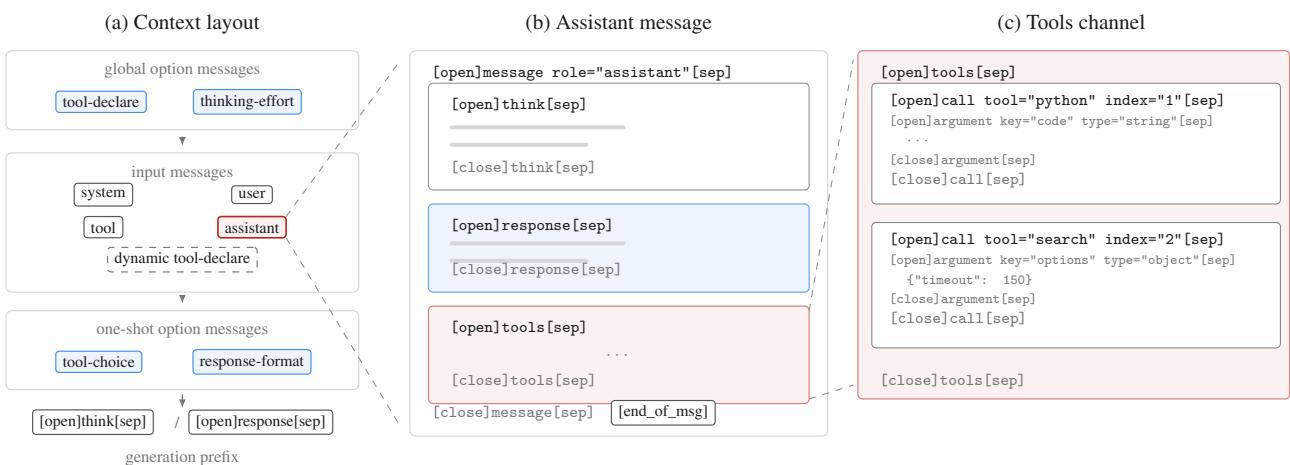
\includegraphics[keepaspectratio,alt={image}]{images/50ffd52873e742ade16668c0d69c4baed39b33583bfff8b288399eb1bfdfb456.jpg}}

图 16: Kimi K3 聊天模板的结构。(a) 上下文布局：全局选项消息位于输入消息之前，而单次选项消息紧随其后，因此每次请求的选项不会影响历史 KV 缓存；动态加载的工具以输入选项消息的形式在会话中注入（虚线）。(b) 助手消息的解剖结构：正文组织为思考（think）、回复（response）和工具（tools）通道。(c) 工具通道的展开：并行的工具调用带有索引，以便工具结果能与其调用匹配，且参数带有类型标注。

定理 2 的证明（上界的紧性） 构造路由器输出 \(I^{*}\) 如下：EP rank 0 上的专家不接收任何 token，而其余 \(R-1\) 个 rank 上的所有专家均匀共享所有 token。则所有 \(S \times K \times R\) 个 token 均匀分配给 \(E(R-1)/R\) 个专家，因此每个专家接收 \(\frac{S K R^{2}}{E(R-1)}\) 个 token。在任意方案 \(P\) 下，rank 0 必须接收 \(S \times K\) 个 token，这些全是远程 token，且这些 token 至少涉及 \(\frac{S K}{\frac{S K R^{2}}{E(R-1)}} = \frac{E(R-1)}{R^{2}}\) 个不同专家；取上取整，rank 0 需要至少 \(\lceil \frac{E(R-1)}{R^{2}} \rceil\) 个冗余专家，因此 \(M(I^{*}) \geq \lceil \frac{E(R-1)}{R^{2}} \rceil\)。反之，通过使用定理 1 证明中的填充过程并优先按专家迁移 token 来构造方案，可以使每个 rank 上的冗余专家数保持在该值以内，因此等式成立。由于当 R 较大时 \(\lceil \frac{E(R-1)}{R^{2}} \rceil \approx \frac{E}{R}\)，定理 1 的上界本质上是紧的：不存在显著小于 \(E/R\) 的通用上界。

\subsection{F 聊天模板}\label{f-chat-template}

Kimi K3 的聊天模板围绕三个目标重新设计。第一是可扩展性：新能力应通过向后兼容的消息格式而非模板修订来引入，使得单一模板服务于整个模型世代。第二是低对齐代价：格式应以最少的监督数据即可学习，支持经过轻度微调的预训练模型可直接进入强化学习的流水线。第三是解码友好性：结构应容纳简单的编码器、流式解析器和语法约束执行器。为此，模板采用 XTML（eXtensible Token Markup Language，可扩展 Token 标记语言），一种类 XML 标记语言，其中尖括号语法被三个保留特殊 token 替代：{[}open{]}、{[}sep{]} 和 {[}close{]}，另有额外的 {[}end\_of\_msg{]} token 作为生成停止标记。元素 {[}open{]}tag attr=``value''{[}sep{]} ... {[}close{]}tag{[}sep{]} 与其 XML 对应物同构，但每个结构边界都是显式的特殊 token，这消除了元素边界处的分词歧义并简化了约束解码。

消息与区域 上下文的顶层单元是消息，消息按来源分为两类（图 16a）。输入消息序列化请求的 messages 字段，涵盖熟悉的 system、user、assistant 和 tool 角色。选项消息将请求选项转化为模型在上下文中读取的指令，其位置反映其作用域。全局选项——工具声明 \(\scriptstyle \left( \mathrm{type = "tool-declare"} \right)\) 和 reasoning-effort 设置——位于所有输入消息之前：它们管理整个会话且很少改变，因此修改它们无论如何都会使 KV 缓存失效。单次选项（tool\_choice、response\_format）追加在输入消息之后，使得每次请求的更改不会影响历史 KV 缓存。第三种类型——输入选项消息——与输入消息交错以补充或覆盖会话中的全局选项。此机制支持动态加载工具：在对话过程中检索或加载的工具通过额外的工具声明消息宣布，此后模型的可用工具集即得到扩展而无需重建前面的上下文。

通道 助手消息的正文组织为通道（channel），这一概念受 OpenAI 的 Harmony 响应格式 {[}85{]} 启发：think 承载推理轨迹，response 承载用户可见的答案，tools 承载工具调用（图 16b）。两种生成模式纯粹通过生成前缀选择——{[}open{]}think{[}sep{]} 用于思考模式，{[}open{]}response{[}sep{]} 用于指令模式——而非通过不同的模板。Kimi K3 仅支持保留式思考：在思考模式下，think 通道始终保留在历史中——即使其内容为空也会保留——以便模型在各轮之间观察到一致的消息结构；在指令模式下，历史消息仅包含 response 和 tools 通道。

工具调用 在 tools 通道内，每次调用携带 tool 和 index 属性；index 编号同一消息内的并行调用，每个工具结果消息重复相同的 tool/index 对并遵循其调用的顺序，从而使结果与调用之间关联明确。参数带有类型标注：字符串参数以原始文本形式出现，而其他 JSON 类型的值则紧凑序列化。因此，诸如代码之类的自由格式文本是一等公民，而非转义的 JSON 字符串。纯 JSON 回退块覆盖那些参数无法分解为带类型参数块的输入；它仅出现在输入 token 中，从不出现在模型输出中，且其损失在训练期间被屏蔽。

推理努力与选项 推理努力以 thinking-effort 类型的全局选项消息暴露，插入在工具声明之后、输入消息之前。该消息不修改生成前缀或暴露 token 预算，而是以自然语言陈述请求的级别，并充当生成约束指令。schema 保留了四个级别（low、medium、high、max），Kimi K3 支持其中的一个子集。这种表示将努力接口与模板语法解耦，并直接与 §4.1.1 和 §4.1.2 中描述的努力条件训练对齐。

更广泛地，这是所有选项消息的共同实现方式：tool\_choice、response\_format 和 thinking-effort 各自被翻译为一段简短的自然语言指令放置在上下文中，而非专用的特殊语法。由于预训练模型已经能够很好地遵循此类指令，新选项可以在很少或无需额外训练的情况下引入——这是上述低对齐代价设计原则的直接体现。
